\chapter{THz Bioeffects: Thermal and Non-Thermal}
\label{ch:thz-bioeffects}

\begin{nontechnical}
\textbf{What is terahertz radiation?}
Think of it as invisible light that sits between microwaves (used in your microwave oven) and infrared (what you feel as heat from the sun). It's completely different from dangerous ionizing radiation like X-rays---THz waves don't have enough energy to damage DNA or cause cancer directly.

\textbf{The Two Types of Effects:}
\begin{enumerate}
\item \textbf{Thermal Effects (Heating)}---\textbf{Well Understood}: THz waves make water molecules jiggle faster, creating heat (like a microwave oven, but much weaker). Only dangerous at high power. Current safety standards keep heating below 1°C---similar to walking from shade into sunlight.

\item \textbf{Non-Thermal Effects (Molecular Resonance?)}---\textbf{Controversial and Unproven}: Some scientists hypothesize that THz might affect biology \emph{without} heating---by vibrating specific molecules at their ``natural frequencies'' (like shattering a wine glass with sound). Most scientists are skeptical; safety standards ignore non-thermal effects because evidence is weak.
\end{enumerate}

\textbf{Should I worry about THz exposure?}
\textbf{No, if exposure is within guidelines.} Current safety limits are conservative---they're set well below levels that cause heating. THz technology is probably safe at low power, but research continues.
\end{nontechnical}

\section{Overview}

Terahertz (THz) radiation (0.1--10 THz) interacts with biological systems through \textbf{thermal} (heating) and potentially \textbf{non-thermal} (resonant or quantum) mechanisms. Understanding these effects is critical for:
\begin{itemize}
\item \textbf{Safety standards}: Protecting workers and patients from excessive exposure
\item \textbf{Medical imaging}: Exploiting THz transparency of clothing for security screening
\item \textbf{Therapeutic applications}: Investigating potential beneficial effects
\item \textbf{Fundamental biophysics}: Understanding molecule-THz interactions
\end{itemize}

\begin{keyconcept}
\textbf{Current consensus}: Thermal effects are well-established and quantifiable. Non-thermal effects remain controversial, with no robust mechanism or reproducible evidence. Safety standards are based exclusively on preventing thermal damage ($\Delta T < 1°$C).
\end{keyconcept}

THz waves are strongly absorbed by water ($\alpha \approx 200$ cm$^{-1}$ at 1 THz), resulting in penetration depths of only $\sim 50$ µm in biological tissue.

\section{Thermal Effects (Established Mechanisms)}

\subsection{Absorption and Heating}

\textbf{Mechanism}: THz radiation absorbed by tissue $\rightarrow$ molecular kinetic energy $\rightarrow$ temperature rise.

The \textbf{heat diffusion equation} governs thermal effects:
\begin{equation}
\rho c_p \frac{\partial T}{\partial t} = \nabla \cdot (k \nabla T) + Q
\end{equation}
where:
\begin{itemize}
\item $\rho$ = tissue density ($\approx 1$ g/cm$^3$)
\item $c_p$ = specific heat capacity ($\approx 3.6$ J/g/K for tissue)
\item $k$ = thermal conductivity ($\approx 0.5$ W/m/K)
\item $Q = \alpha I$ = volumetric heat generation rate (W/cm$^3$)
\item $\alpha$ = absorption coefficient (cm$^{-1}$)
\item $I$ = local intensity (W/cm$^2$)
\end{itemize}

For \textbf{steady-state temperature rise} (no blood flow):
\begin{equation}
\Delta T \approx \frac{\alpha I \delta^2}{k}
\end{equation}
where:
\begin{itemize}
\item $\delta = 1/\alpha$ = penetration depth
\item At 1 THz: $\alpha \approx 200$ cm$^{-1}$, $\delta \approx 50$ µm
\end{itemize}

\textbf{Numerical example} (1 THz exposure):
\begin{equation}
\Delta T \approx \frac{(200 \times 10^4\,\text{m}^{-1}) \times (10^4\,\text{W/m}^2) \times (50 \times 10^{-6}\,\text{m})^2}{0.5\,\text{W/m/K}} \approx 1°\text{C}
\end{equation}

This shows that 1 W/cm$^2$ exposure produces $\sim$1°C heating---the \textbf{safety threshold}.

\subsection{Penetration Depth and Frequency Dependence}

The \textbf{Beer-Lambert law} describes intensity attenuation:
\begin{equation}
I(z) = I_0 e^{-\alpha z}
\end{equation}
where:
\begin{itemize}
\item $I_0$ = incident intensity at surface
\item $z$ = depth into tissue
\item $\alpha(f)$ = frequency-dependent absorption coefficient
\end{itemize}

Absorption coefficient for water:
\begin{equation}
\alpha(f) \approx 0.5 f^2 \quad \text{(cm}^{-1}\text{, } f \text{ in THz)}
\end{equation}

Penetration depth:
\begin{equation}
\delta(f) = \frac{1}{\alpha(f)} \approx \frac{2}{f^2} \quad \text{(cm)}
\end{equation}

\begin{center}
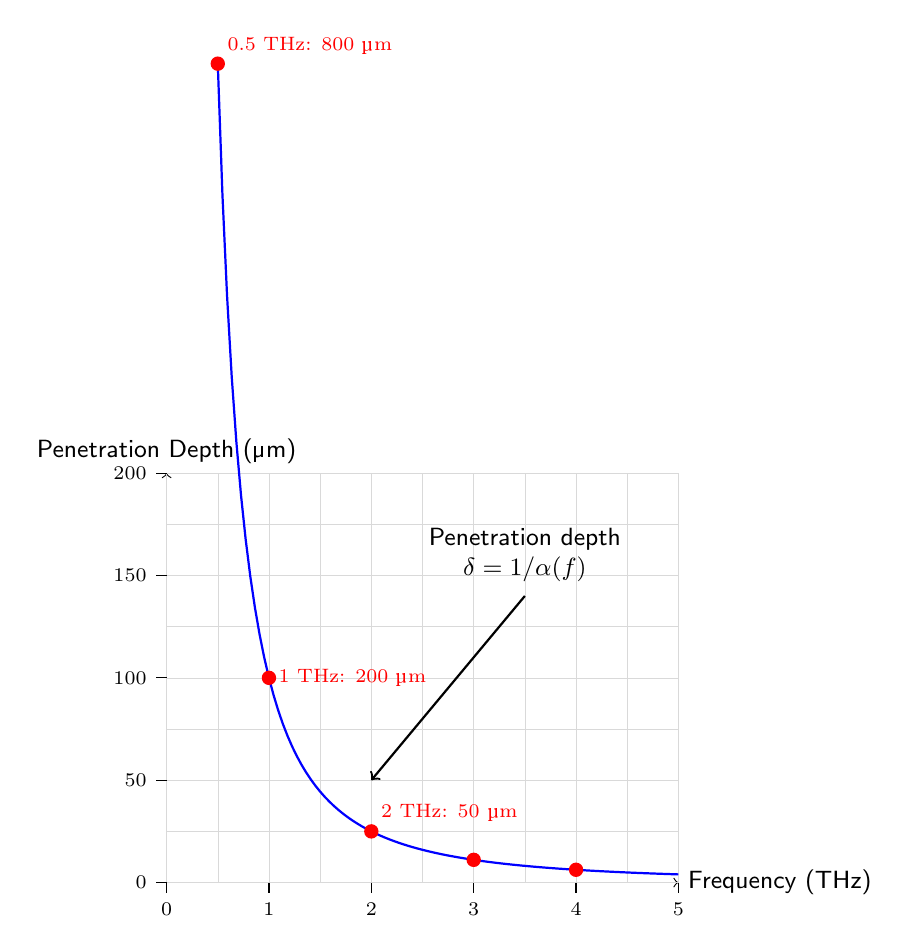
\begin{tikzpicture}[scale=1.3]
% Axes
\draw[->] (0,0) -- (5,0) node[right] {\sffamily\small Frequency (THz)};
\draw[->] (0,0) -- (0,4) node[above] {\sffamily\small Penetration Depth (µm)};

% Grid
\draw[very thin,gray!30] (0,0) grid[step=0.5] (5,4);

% Tick marks and labels
\foreach \x in {0,1,2,3,4,5}
  \draw (\x,0) -- (\x,-0.1) node[below,font=\scriptsize] {\x};
\foreach \y in {0,50,100,150,200}
  \draw (0,{\y/50}) -- (-0.1,{\y/50}) node[left,font=\scriptsize] {\y};

% Penetration depth curve (δ ∝ 1/f²)
\draw[thick,blue] plot[domain=0.5:5,samples=100] (\x,{2/(\x*\x)});

% Key frequency markers
\fill[red] (0.5,{2/(0.5*0.5)}) circle (2pt) node[above right,font=\scriptsize] {0.5 THz: 800 µm};
\fill[red] (1,2) circle (2pt) node[right,font=\scriptsize] {1 THz: 200 µm};
\fill[red] (2,0.5) circle (2pt) node[above right,font=\scriptsize] {2 THz: 50 µm};
\fill[red] (3,{2/9}) circle (2pt);
\fill[red] (4,{2/16}) circle (2pt);

% Annotation
\node[align=center,font=\sffamily\small] at (3.5,3.2) {Penetration depth\\$\delta = 1/\alpha(f)$};
\draw[->,thick] (3.5,2.8) -- (2,1);
\end{tikzpicture}
\end{center}

\textbf{Implications}:
\begin{itemize}
\item Lower frequencies (0.1--0.5 THz) penetrate deeper $\rightarrow$ bulk heating
\item Higher frequencies ($>$2 THz) confined to surface $\rightarrow$ skin-only effects
\item Medical imaging typically uses 0.1--1 THz for optimal tissue contrast
\end{itemize}

\subsection{Heat Diffusion Visualization}

The spatial temperature distribution follows:

\begin{center}
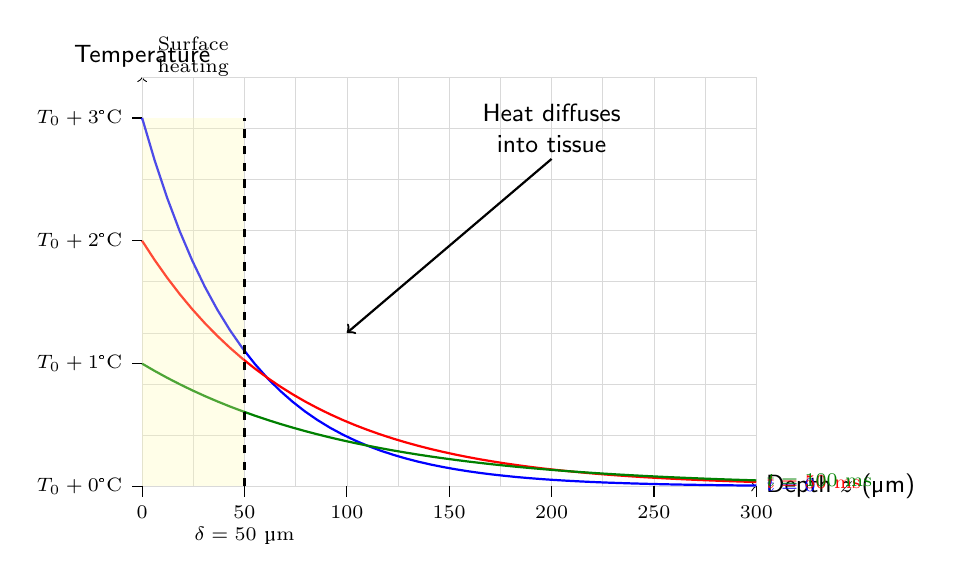
\begin{tikzpicture}[scale=1.3]
% Surface and depth axis
\draw[->] (0,0) -- (6,0) node[right] {\sffamily\small Depth $z$ (µm)};
\draw[->] (0,0) -- (0,4) node[above] {\sffamily\small Temperature};

% Grid
\draw[very thin,gray!30] (0,0) grid[step=0.5] (6,4);

% Tick marks
\foreach \x in {0,50,100,150,200,250,300}
  \draw ({\x/50},0) -- ({\x/50},-0.1) node[below,font=\scriptsize] {\x};
\foreach \y in {0,1,2,3}
  \draw (0,{1.2*\y}) -- (-0.1,{1.2*\y}) node[left,font=\scriptsize] {$T_0+\y$°C};

% Exponential decay curves for different times
\draw[thick,blue] plot[domain=0:6,samples=50] (\x,{3.6*exp(-\x/1)}) node[right,font=\scriptsize] {$t=0$};
\draw[thick,red] plot[domain=0:6,samples=50] (\x,{2.4*exp(-\x/1.5)}) node[right,font=\scriptsize] {$t=50$ ms};
\draw[thick,green!50!black] plot[domain=0:6,samples=50] (\x,{1.2*exp(-\x/2)}) node[right,font=\scriptsize] {$t=100$ ms};

% Surface heating zone
\fill[yellow!30,opacity=0.3] (0,0) rectangle (1,3.6);
\node[font=\scriptsize,align=center] at (0.5,4.2) {Surface\\heating};

% Penetration depth marker
\draw[thick,dashed] (1,0) -- (1,3.6);
\node[below,font=\scriptsize] at (1,-0.3) {$\delta = 50$ µm};

% Annotation
\node[align=center,font=\sffamily\small] at (4,3.5) {Heat diffuses\\into tissue};
\draw[->,thick] (4,3.2) -- (2,1.5);
\end{tikzpicture}
\end{center}

\subsection{Thermal Diffusion Time}

Heat dissipation is governed by thermal diffusion:
\begin{equation}
\tau_{\text{th}} = \frac{L^2}{\kappa}
\end{equation}
where:
\begin{itemize}
\item $\kappa = k/(\rho c_p)$ = thermal diffusivity ($\approx 1.3 \times 10^{-3}$ cm$^2$/s for tissue)
\item $L$ = characteristic length scale
\end{itemize}

For $L = 100$ µm:
\begin{equation}
\tau_{\text{th}} = \frac{(100 \times 10^{-6}\,\text{m})^2}{1.3 \times 10^{-7}\,\text{m}^2/\text{s}} \approx 0.077\,\text{s}
\end{equation}

\begin{calloutbox}{Pulsed vs. Continuous Wave (CW) Exposure}
\textbf{Short pulses} ($<< \tau_{\text{th}}$): Create transient temperature spikes that relax before tissue damage. Peak temperature may exceed steady-state values.

\textbf{Long pulses or CW} ($>> \tau_{\text{th}}$): Reach thermal equilibrium. Safety limits based on average power.

\textbf{Duty cycle matters}: A 1 ms pulse at 100 W/cm$^2$ repeated every 1 s (0.1\% duty cycle) has same average heating as 0.1 W/cm$^2$ CW---but peak temperature differs!
\end{calloutbox}

\subsection{Biological Consequences of Heating}

Temperature rise determines biological response:

\begin{center}
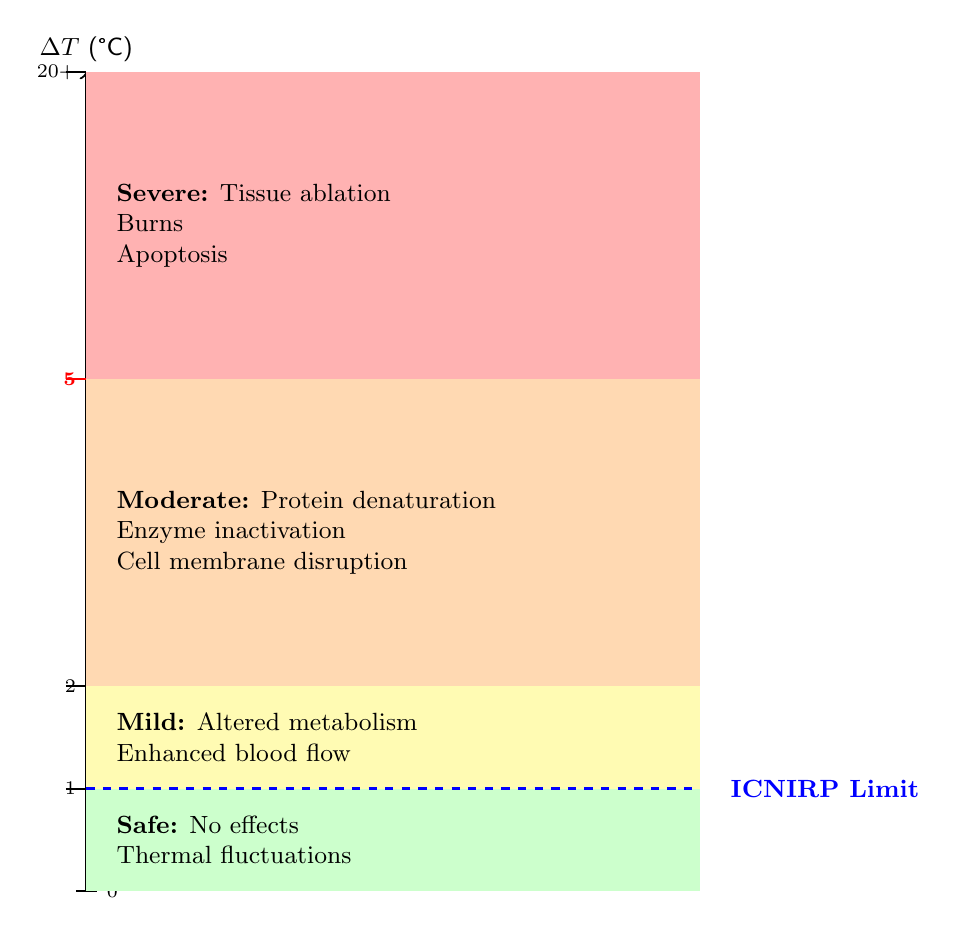
\begin{tikzpicture}[scale=1.3]
% Temperature scale
\draw[thick,->] (0,0) -- (0,8) node[above] {\sffamily\small $\Delta T$ (°C)};
\draw[thick] (-0.1,0) -- (0.1,0) node[right] {\scriptsize 0};

% Zones with different effects
\fill[green!20] (0,0) rectangle (6,1);
\fill[yellow!30] (0,1) rectangle (6,2);
\fill[orange!30] (0,2) rectangle (6,5);
\fill[red!30] (0,5) rectangle (6,8);

% Zone labels
\node[right,align=left,font=\small] at (0.2,0.5) {\textbf{Safe:} No effects\\Thermal fluctuations};
\node[right,align=left,font=\small] at (0.2,1.5) {\textbf{Mild:} Altered metabolism\\Enhanced blood flow};
\node[right,align=left,font=\small] at (0.2,3.5) {\textbf{Moderate:} Protein denaturation\\Enzyme inactivation\\Cell membrane disruption};
\node[right,align=left,font=\small] at (0.2,6.5) {\textbf{Severe:} Tissue ablation\\Burns\\Apoptosis};

% Temperature markers
\draw[thick] (-0.2,1) -- (0,1) node[left] {\scriptsize 1};
\draw[thick] (-0.2,2) -- (0,2) node[left] {\scriptsize 2};
\draw[thick,red] (-0.2,5) -- (0,5) node[left] {\scriptsize\textbf{5}};
\draw[thick] (-0.2,8) -- (0,8) node[left] {\scriptsize 20+};

% ICNIRP limit
\draw[blue,very thick,dashed] (0,1) -- (6,1);
\node[right,blue,font=\small\bfseries] at (6.2,1) {ICNIRP Limit};
\end{tikzpicture}
\end{center}

\textbf{Key thresholds}:
\begin{itemize}
\item $\Delta T < 1°$C: No adverse effects (ICNIRP safety limit)
\item $\Delta T = 1$--2°C: Mild heating, increased metabolic rate
\item $\Delta T = 5$--10°C: Protein denaturation begins (irreversible above $\sim$43°C absolute)
\item $\Delta T > 20°$C: Tissue ablation, burns
\end{itemize}

\section{Non-Thermal Effects (Speculative Mechanisms)}

\subsection{Definition and Challenge}

\textbf{Non-thermal effect}: Biological response that occurs at intensities too low to cause measurable heating ($\Delta T < 0.1°$C) OR that persists after heating stops.

\begin{center}
\begin{tikzpicture}[
  block/.style={rectangle, draw, minimum width=3cm, minimum height=1.2cm, font=\sffamily\small, align=center},
  node distance=2.5cm,
  font=\small
]
% Top: THz Exposure
\node[block,fill=yellow!20] (thz) {THz Radiation\\$I, f$};

% Two pathways
\node[block,fill=red!20,below left=1.5cm and 1.5cm of thz] (thermal) {Thermal\\Mechanism};
\node[block,fill=blue!20,below right=1.5cm and 1.5cm of thz] (nonthermal) {Non-Thermal?\\Mechanism};

% Thermal pathway details
\node[block,below=1.2cm of thermal,font=\scriptsize] (heat) {Absorption $\rightarrow$\\Heat Generation\\$Q = \alpha I$};
\node[block,below=1.2cm of heat,font=\scriptsize] (temprise) {Temperature\\Rise\\$\Delta T$};
\node[block,below=1.2cm of temprise,font=\scriptsize,fill=green!20] (damage) {Cell Damage\\if $\Delta T > 1°$C};

% Non-thermal pathway details
\node[block,below=1.2cm of nonthermal,font=\scriptsize] (resonance) {Resonant\\Excitation?\\Membrane?};
\node[block,below=1.2cm of resonance,font=\scriptsize] (signal) {Signaling\\Cascade?};
\node[block,below=1.2cm of signal,font=\scriptsize,fill=orange!20] (effect) {Biological\\Effect?};

% Arrows
\draw[->,thick] (thz) -- (thermal);
\draw[->,thick] (thz) -- (nonthermal);
\draw[->,thick] (thermal) -- (heat);
\draw[->,thick] (heat) -- (temprise);
\draw[->,thick] (temprise) -- (damage);
\draw[->,thick,dashed] (nonthermal) -- (resonance);
\draw[->,thick,dashed] (resonance) -- (signal);
\draw[->,thick,dashed] (signal) -- (effect);

% Labels
\node[font=\tiny\bfseries,red] at (-2.5,-4) {ESTABLISHED};
\node[font=\tiny\bfseries,blue] at (2.5,-4) {CONTROVERSIAL};

% Question marks
\node[font=\Large,blue] at (3,-2.5) {?};
\node[font=\Large,blue] at (3,-4.5) {?};
\node[font=\Large,blue] at (3,-6.5) {?};

\end{tikzpicture}
\end{center}

\begin{warningbox}
Distinguishing true non-thermal effects from thermal artifacts is extremely difficult:
\begin{itemize}
\item \textbf{Localized heating}: Field enhancement at sharp features (cell edges, organelles) creates ``hot spots'' below measurement resolution
\item \textbf{Transient heating}: Temporary temperature spikes below detection threshold ($<$0.01°C)
\item \textbf{Indirect thermal effects}: Heat-activated signaling cascades with long time constants
\end{itemize}
Many claimed ``non-thermal'' effects are likely subtle thermal phenomena.
\end{warningbox}

\subsection{Proposed Mechanisms}

\subsubsection{Resonant Absorption by Biomolecules}

\textbf{Hypothesis}: THz frequencies match vibrational modes of proteins, DNA, or membranes $\rightarrow$ selective excitation.

Proteins have collective vibrational modes:
\begin{equation}
\omega_{\text{vib}} = \sqrt{\frac{k_{\text{eff}}}{m_{\text{eff}}}}
\end{equation}
where:
\begin{itemize}
\item $k_{\text{eff}}$ = effective spring constant of hydrogen bonds ($\sim$10 N/m)
\item $m_{\text{eff}}$ = effective mass of amino acid residues
\item Typical frequencies: 0.1--3 THz (low-frequency Raman, THz-TDS)
\end{itemize}

\textbf{Problem}: In aqueous solution, these modes are heavily broadened (lifetime $\sim$ ps) due to solvent damping $\rightarrow$ weak resonance peak. Excitation is non-selective.

\textbf{Linewidth} of resonance:
\begin{equation}
\Gamma = \frac{1}{\pi \tau} \approx \frac{1}{\pi \times 10^{-12}\,\text{s}} \approx 0.3\,\text{THz}
\end{equation}

This broad linewidth ($\Delta f / f \approx 30$\%) makes selective excitation unlikely.

\subsubsection{Membrane Electroporation}

\textbf{Hypothesis}: THz electric fields induce transmembrane voltage $\rightarrow$ pore formation.

Induced voltage across cell membrane:
\begin{equation}
V_m = 1.5 r E \cos\theta
\end{equation}
where:
\begin{itemize}
\item $r$ = cell radius
\item $E$ = external electric field
\item $\theta$ = angle from field direction
\end{itemize}

For $r = 10$ µm, $E = 10$ kV/cm:
\begin{equation}
V_m \approx 1.5 \times (10 \times 10^{-6}\,\text{m}) \times (10^6\,\text{V/m}) = 15\,\text{mV}
\end{equation}

\textbf{Electroporation threshold}: $V_m \approx 1$ V (requires $E \sim$ 1 MV/cm).

\textbf{Conclusion}: THz fields are shielded by ionic double layer; frequency too high for membrane charging. Electroporation unlikely at achievable THz intensities.

\subsubsection{Microtubule Resonances}

\textbf{Hypothesis}: THz resonates with microtubule vibrational modes $\rightarrow$ alters quantum coherence $\rightarrow$ affects neural function.

Predicted resonance frequencies (Fröhlich model):
\begin{equation}
f_n = \frac{v_s}{2\pi R} \sqrt{n^2 + m^2}
\end{equation}
where:
\begin{itemize}
\item $v_s$ = sound velocity in microtubule ($\approx 1.5 \times 10^3$ m/s)
\item $R$ = microtubule radius ($\approx 12$ nm)
\item $n, m$ = mode numbers
\end{itemize}

Fundamental mode ($n=1, m=0$):
\begin{equation}
f_1 \approx \frac{1.5 \times 10^3}{2\pi \times 12 \times 10^{-9}} \approx 20\,\text{GHz}
\end{equation}

Higher harmonics reach THz range, but damping increases with frequency.

\textbf{Status}: No direct experimental test; theoretical models exist but lack validation.

\subsubsection{Water Structuring}

\textbf{Hypothesis}: THz alters hydrogen bond network dynamics in vicinal water (near protein/membrane surfaces) $\rightarrow$ affects protein function.

THz drives librational modes (hindered rotations) of water:
\begin{equation}
\omega_{\text{lib}} \approx \sqrt{\frac{3k_BT}{I}} \approx 2\pi \times 1\,\text{THz}
\end{equation}
where:
\begin{itemize}
\item $k_B$ = Boltzmann constant
\item $T$ = temperature
\item $I$ = moment of inertia of H$_2$O molecule
\end{itemize}

\textbf{Mechanism}: THz transiently disrupts H-bond network $\rightarrow$ lowers activation barrier for protein conformational changes.

\textbf{Evidence}: Simulations suggest THz can perturb water structure on $\sim$ ps timescales; biological relevance unclear.

\section{Experimental Evidence}

\subsection{Cell-Level Studies}

\textbf{Gene expression}:
\begin{itemize}
\item \textbf{Observation}: Altered mRNA levels after THz exposure (0.1--2.5 THz, $<$1 mW/cm$^2$, $<$1°C heating)
\item \textbf{Example}: Upregulation of heat shock proteins (HSP70) in human keratinocytes (Wilmink et al., 2010)
\item \textbf{Interpretation}: Could be indirect thermal effect (transient microheating) OR non-thermal stress response
\end{itemize}

\textbf{Membrane permeability}:
\begin{itemize}
\item \textbf{Observation}: Increased uptake of fluorescent dyes after THz pulse exposure (Bock et al., 2010)
\item \textbf{Interpretation}: Pore formation? Or thermal disruption?
\item \textbf{Control needed}: Measure temperature with high spatial/temporal resolution
\end{itemize}

\textbf{Calcium signaling}:
\begin{itemize}
\item \textbf{Observation}: Transient Ca$^{2+}$ influx in neurons after THz exposure (Zhao et al., 2019)
\item \textbf{Mechanism}: THz-sensitive ion channels? Or indirect heating?
\item \textbf{Problem}: Calcium-sensitive dyes themselves have temperature dependence
\end{itemize}

\subsection{Critical Analysis: Are Non-Thermal Effects Real?}

\textbf{Arguments For}:
\begin{enumerate}
\item Molecular resonances exist: Proteins, DNA have THz vibrational modes
\item Some cellular effects at low intensity: Not all studies show strict temperature correlation
\item Precedent in other bands: RF/microwave ``non-thermal effects'' debated for decades
\end{enumerate}

\textbf{Arguments Against}:
\begin{enumerate}
\item No consensus mechanism: Multiple proposed mechanisms, none with strong evidence
\item Reproducibility issues: Many studies lack independent replication
\item Thermal artifacts: Hard to rule out localized or transient heating
\item Lack of dose-response: No clear threshold or saturation behavior for ``non-thermal'' effects
\item Evolutionary perspective: If THz resonances were functionally important, natural selection would have exploited or shielded them
\end{enumerate}

\begin{calloutbox}{Current Scientific Consensus}
\textbf{ICNIRP position} (2013): ``There is no consistent evidence for non-thermal effects at intensities below thermal damage thresholds.''

\textbf{WHO position}: THz safety guidelines based on thermal effects only.

\textbf{Research community}: Divided; ongoing studies but skepticism high.
\end{calloutbox}

\section{Safety Standards}

\subsection{ICNIRP Guidelines (2013)}

\textbf{Frequency range}: 0.3--3 THz

\textbf{Power density limits}:
\begin{itemize}
\item \textbf{Occupational exposure}: $S_{\text{occ}} = 10$ mW/cm$^2$\\
(averaged over $68/f^{1.05}$ minutes, where $f$ is in THz)
\item \textbf{General public exposure}: $S_{\text{pub}} = 2$ mW/cm$^2$ (same averaging)
\end{itemize}

\textbf{Rationale}: Keep $\Delta T < 1°$C.

\begin{center}
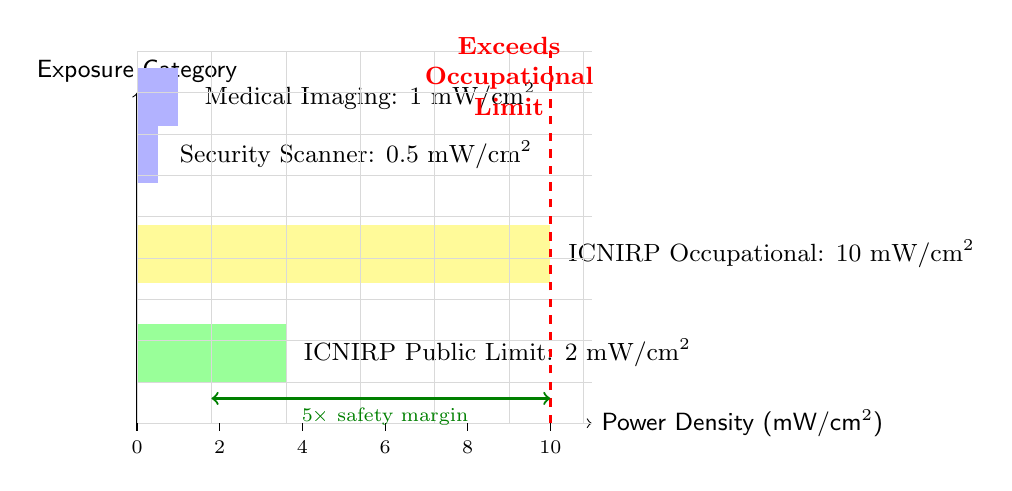
\begin{tikzpicture}[scale=1.05]
% Axes
\draw[->] (0,0) -- (5.5,0) node[right] {\sffamily\small Power Density (mW/cm$^2$)};
\draw[->] (0,0) -- (0,4) node[above] {\sffamily\small Exposure Category};

% Bars for different exposure categories
% Safe zone (0-2)
\fill[green!40] (0,0.5) rectangle (1.8,1.2);
\node[right,font=\small] at (1.9,0.85) {ICNIRP Public Limit: 2 mW/cm$^2$};

% Occupational (0-10)
\fill[yellow!40] (0,1.7) rectangle (10/2,2.4);
\node[right,font=\small] at (5.1,2.05) {ICNIRP Occupational: 10 mW/cm$^2$};

% Typical applications
\fill[blue!30] (0,2.9) rectangle (0.5/2,3.6);
\node[right,font=\small] at (0.4,3.25) {Security Scanner: 0.5 mW/cm$^2$};

\fill[blue!30] (0,3.6) rectangle (1/2,4.3);
\node[right,font=\small] at (0.7,3.95) {Medical Imaging: 1 mW/cm$^2$};

% Grid lines
\draw[very thin,gray!30] (0,0) grid[xstep=0.9,ystep=0.5] (5.5,4.5);

% X-axis ticks
\foreach \x in {0,2,4,6,8,10}
  \draw ({\x/2},0) -- ({\x/2},-0.1) node[below,font=\scriptsize] {\x};

% Danger zone marker
\draw[red,very thick,dashed] (10/2,0) -- (10/2,4.5);
\node[red,font=\small\bfseries,align=center] at (4.5,4.2) {Exceeds\\Occupational\\Limit};

% Safe margin annotation
\draw[<->,thick,green!50!black] (1.8/2,0.3) -- (10/2,0.3);
\node[below,font=\scriptsize,green!50!black] at (3.0,0.3) {5× safety margin};

\end{tikzpicture}
\end{center}

Time-averaged power density:
\begin{equation}
S_{\text{avg}} = \frac{1}{T} \int_0^T S(t) \, dt < S_{\text{limit}}
\end{equation}

\subsection{IEEE Standards (C95.1-2019)}

Similar limits: $\sim$10 mW/cm$^2$ for controlled environments.

\textbf{Frequency gaps}: Standards less developed for 3--10 THz (far-IR overlap).

\subsection{Medical Device Regulations}

\textbf{THz imaging systems}: Require FDA clearance (USA) or CE mark (EU).

\textbf{Approval criteria}:
\begin{itemize}
\item Demonstrate temperature rise $<$1°C in vivo
\item No evidence of long-term effects (mutagenicity, carcinogenicity)
\end{itemize}

\section{Worked Example: Safety Compliance Check}

\textbf{Problem}: A THz security scanner operates at 0.5 THz with 5 mW average power, beam area 10 cm$^2$, scan time 2 seconds per person. Is this safe for public use?

\textbf{Given}:
\begin{itemize}
\item Frequency: $f = 0.5$ THz
\item Average power: $P = 5$ mW
\item Beam area: $A = 10$ cm$^2$
\item Exposure time: $t = 2$ s
\end{itemize}

\textbf{Required}: Compare to ICNIRP public exposure limit.

\textbf{Solution}:

\textit{Step 1: Calculate average power density}
\begin{equation}
S_{\text{avg}} = \frac{P}{A} = \frac{5\,\text{mW}}{10\,\text{cm}^2} = 0.5\,\text{mW/cm}^2
\end{equation}

\textit{Step 2: Find ICNIRP limit for public at 0.5 THz}

ICNIRP public limit:
\begin{equation}
S_{\text{pub}} = 2\,\text{mW/cm}^2
\end{equation}
(averaged over $68/f^{1.05} = 68/0.5^{1.05} \approx 132$ minutes)

\textit{Step 3: Compare}
\begin{equation}
\frac{S_{\text{avg}}}{S_{\text{pub}}} = \frac{0.5}{2} = 0.25 = 25\%
\end{equation}

\textbf{Answer}: The scanner operates at 25\% of the ICNIRP public exposure limit.

\textbf{Interpretation}: This is well within safety guidelines. Even with 2-second exposure, no averaging needed since instantaneous power density (0.5 mW/cm$^2$) is below the limit. Temperature rise would be:
\begin{equation}
\Delta T \approx \frac{\alpha S_{\text{avg}} \delta^2}{k} = \frac{(100\,\text{cm}^{-1}) \times (0.5 \times 10^{-3}\,\text{W/cm}^2) \times (0.01\,\text{cm})^2}{0.005\,\text{W/cm/K}} \approx 0.01°\text{C}
\end{equation}

This is negligible compared to natural thermal fluctuations.

\section{Applications}

\subsection{THz Security Screening}

THz waves penetrate clothing but not skin $\rightarrow$ detect concealed objects without ionizing radiation.

\textbf{Technology}:
\begin{itemize}
\item Frequency: 0.1--0.5 THz (balance penetration vs. resolution)
\item Power: $<$1 mW (well below safety limits)
\item Imaging: Raster scan or focal plane arrays
\end{itemize}

\textbf{Safety advantage}: No ionizing radiation; 100× lower power than mobile phones.

\subsection{THz Medical Imaging}

\textbf{Applications}:
\begin{itemize}
\item Skin cancer detection: THz reflection spectroscopy distinguishes malignant tissue (different water content)
\item Burn depth assessment: Penetration depth matches dermis thickness
\item Dental imaging: Non-ionizing alternative to X-rays
\end{itemize}

\textbf{Challenges}:
\begin{itemize}
\item Limited penetration ($<$1 mm) $\rightarrow$ surface-only imaging
\item Long acquisition times (raster scanning)
\item Competition from ultrasound, OCT
\end{itemize}

\subsection{THz Spectroscopy in Pharmaceutical QC}

\textbf{Application}: Non-destructive analysis of tablet composition, coating uniformity.

\textbf{Advantage}: THz absorption spectra are molecular ``fingerprints'' (unlike X-rays, which are density-based).

\textbf{Safety}: Reflection-mode measurement; no thermal effects on samples.

\section{Summary}

\begin{center}
\begin{tabular}{ll}
\toprule
\textbf{Parameter} & \textbf{Value/Description} \\
\midrule
THz frequency range & 0.1--10 THz \\
Penetration depth (1 THz) & $\sim$50 µm (skin surface only) \\
Absorption mechanism & Water molecule vibrations \\
Thermal diffusion time & $\sim$0.1 s (for 100 µm depth) \\
ICNIRP occupational limit & 10 mW/cm$^2$ (averaged) \\
ICNIRP public limit & 2 mW/cm$^2$ (averaged) \\
Safety threshold & $\Delta T < 1°$C \\
Non-thermal effects & Controversial, no consensus \\
\bottomrule
\end{tabular}
\end{center}

\textbf{Advantages of Thermal Model}:
\begin{itemize}
\item Quantifiable and predictable
\item Well-tested experimentally
\item Basis for international safety standards
\item Conservative approach protects public health
\end{itemize}

\textbf{Disadvantages / Unknowns}:
\begin{itemize}
\item Cannot rule out subtle non-thermal effects
\item Long-term exposure data limited (technology relatively new)
\item High-frequency regime (3--10 THz) less studied
\end{itemize}

\textbf{Best suited for}: Low-power, short-duration applications (security screening, medical imaging, spectroscopy) where thermal effects are negligible.

\section{Further Reading}

\begin{itemize}
\item For THz absorption spectra: Chapter~\ref{ch:thz-propagation} (THz Propagation in Biological Tissue)
\item For speculative quantum mechanisms: Chapter~\ref{ch:thz-microtubules} (THz Resonances in Microtubules)
\item For THz technology: Chapter~\ref{ch:thz-technology} (Terahertz Technology: Sources and Detectors)
\item For related RF phenomena: Chapter~\ref{ch:frey-effect} (Frey Microwave Auditory Effect)
\end{itemize}

\section{References}

\subsection{Thermal Effects (Established)}

\begin{enumerate}
\item \textbf{ICNIRP, \emph{Health Phys.} 105, 171 (2013)} --- THz exposure guidelines
\item \textbf{Pickwell \& Wallace, \emph{J. Phys. D} 39, R301 (2006)} --- THz-tissue interactions
\end{enumerate}

\subsection{Non-Thermal Effects (Speculative)}

\textbf{To definitively test non-thermal hypotheses:}
\begin{enumerate}
\setcounter{enumi}{2}
\item \textbf{Wilmink et al., \emph{J. Infrared Millim. THz Waves} 31, 1234 (2010)} --- Gene expression changes
\item \textbf{Titova et al., \emph{Sci. Rep.} 3, 2363 (2013)} --- Zebrafish developmental effects
\item \textbf{Zhao et al., \emph{Neurophotonics} 6, 011004 (2019)} --- Calcium signaling in neurons
\end{enumerate}

\subsection{Critical Reviews}

\begin{enumerate}
\setcounter{enumi}{5}
\item \textbf{Alexandrov et al., \emph{Phys. Lett. A} 374, 1214 (2010)} --- DNA resonances (controversial)
\item \textbf{Foster, \emph{Radiat. Res.} 162, 492 (2004)} --- Critique of non-thermal RF/THz effects
\end{enumerate}

\subsection{Vibronic Coupling}

\textbf{Related chapters in this book:}
\begin{itemize}
\item Chapter~\ref{ch:thz-technology}: THz sources, detectors, and applications
\item Chapter~\ref{ch:thz-propagation}: Absorption, scattering, and penetration in biological tissue
\item Chapter~\ref{ch:thz-resonances}: Microtubule vibrational modes and quantum hypothesis
\item Chapter~\ref{ch:quantum-coherence}: Quantum effects in biology (photosynthesis, magnetoreception, neural coherence)
\item Chapter~\ref{ch:frey-effect}: Analogous non-thermal RF effect (pulsed microwave auditory perception)
\end{itemize}

\textbf{Key references:}
\begin{enumerate}
\item ICNIRP, ``Guidelines for limiting exposure to electromagnetic fields (100~kHz to 300~GHz),'' \textit{Health Physics} \textbf{118}, 483--524 (2020)
\item Pickwell \& Wallace, ``Biomedical applications of terahertz technology,'' \textit{J. Phys. D: Appl. Phys.} \textbf{39}, R301--R310 (2006)
\item Wilmink et al., ``Development of a compact terahertz time-domain spectrometer for the measurement of the optical properties of biological tissues,'' \textit{J. Biomed. Opt.} \textbf{16}, 047006 (2011)
\item Foster, ``Thermal and nonthermal mechanisms of interaction of radio-frequency energy with biological systems,'' \textit{IEEE Trans. Plasma Sci.} \textbf{28}, 15--23 (2000)
\item Bao et al., ``Vibronically coherent ultrafast triplet-pair formation and subsequent thermally activated dissociation control efficient endothermic singlet fission,'' \textit{J. Chem. Theory Comput.} \textbf{20}, 4377--4389 (2024)
\end{enumerate}

\textbf{Critical reviews:}
\begin{itemize}
\item Alexandrov et al., ``DNA breathing dynamics in the presence of a terahertz field,'' \textit{Phys. Lett. A} \textbf{374}, 1214--1217 (2010) [Controversial; replication failed]
\item Romanenko et al., ``The interaction between electromagnetic fields at megahertz, gigahertz and terahertz frequencies with cells, tissues and organisms: Risks and potential,'' \textit{J. R. Soc. Interface} \textbf{14}, 20170585 (2017) [Comprehensive critical review]
\end{itemize}
